\documentclass[
  % all of the below options are optional and can be left out
  % course name (default: 2IL50 Data Structures)
  course = {{IE579 Game Theory and Multi-Agent Reinforcement Learning}},
  % quartile (default: 3)
  quartile = {{4}},
  % assignment number/name (default: 1)
  assignment = 2,
  % student name (default: Some One)
  name = {{Mohammad Mahdi Rahimi}},
  % student number, NOT S-number (default: 0123456)
  studentnumber = {{20208244}},
  % student email (default: s.one@student.tue.nl)
  email = {{mahi@kaist.ac.kr}},
  % first exercise number (default: 1)
  firstexercise = 1
]{aga-homework}

\usepackage{amssymb,latexsym,amsmath,amsthm}
\usepackage{amsfonts,rawfonts}
\usepackage{thmtools}
\usepackage{systeme}
\usepackage{mathtools}
\usepackage{xcolor}
\usepackage{pgfplots} 
\usepackage{amsmath}
\usepackage{algorithm}
\usepackage{cancel}
\usepackage[noend]{algpseudocode}
\usepackage{minted}
\usepackage{tikz}
\usetikzlibrary{calc}
\usepackage[dvipsnames]{xcolor}
% \usepackage[margin=1.5in]{geometry}    % For margin alignment


\pgfplotsset{width=10cm,compat=1.9} 
 \usepgfplotslibrary{external}

\tikzexternalize 
% \tikzset{
%   % Two node styles for game trees: solid and hollow
%   solid node/.style={circle,draw,inner sep=2,fill=black},
%   hollow node/.style={circle,draw,inner sep=2},
%   empty node/.style={rectangle,draw,fill=white,color=white}
% }

% macro for entering payoffs
\newcommand\payoff[1]{
  $\begin{pmatrix} #1 \end{pmatrix}$
}



\begin{document}

\exercise
\subexercise $x = 1$ Find Pure Nash and SPE
\\\\
Nash Equilibrium :\\
1. \{(R,G),(U)\}\\
2. \{(R,H),(U)\}\\
3. \{(L,G),(D)\}\\
4. \{(L,H),(D)\}\\
\\
Sub-game Perfect Nash Equilibrium :\\
1. \{(R,H),(U)\}


\subexercise Range of x for having (R, U) as unique SPE
\\\\
For $x > 2$ player-1 choose $(L)$, and for $x = 2$ player-1 is indifferent between $(L)$ and $(R)$ in sub-game, so for the range of $x < 2$, $(R, U)$ is the unique SPE.
\\\\
\subexercise  Range of x for having (L) as unique SPE
\\\\
For $x > 2$ player-1 choose $(L)$, and it is the unique SPE.

\exercise
\subexercise All Pure Nash
\\\\
Player-1 Actions: $\{L, C, R\}$\\
Player-2 Actions: $\{U, D\}$\\
Converting game to a normal-form(3x2) we find following pure Nash equilibrium:\\
1. $(R, U) = (5, 5)$\\
2. $(C, D) = (5, 5)$

\subexercise Mixed Nash Equilibrium \\\\
For finding mixed equilibrium we randomize over pure solutions actions:\\
Player-1 Plays: $P\{R\} + (1 - P)\{C\}$\\
Player-2 Plays: $Q\{U\} + (1 - Q)\{D\}$\\
So we get:\\
\begin{equation} \label{eq1}
\begin{split}
& PQ\{R, U\} + (1 - P)Q\{C, U\} + p(1 - Q)\{R, D\} + (1 - P)(1 - Q)\{C, D\} \\
= & PQ\{5, 5\} + (1 - P)Q\{0, 0\} + P(1 - Q)\{-15, -15\} + (1 - P)(1 - Q)\{5, 5\}\\
\Rightarrow &   \begin{cases}
      U_1 = 5PQ + -15P(1 - Q) + 5(1 - P)(1 - Q) = 25PQ - 20P - 5Q + 5 = P(25Q - 20) - 5Q + 5 \\
      U_2 = 5PQ + -15P(1 - Q) + 5(1 - P)(1 - Q) = 25PQ - 20P - 5Q + 5 = Q(25Q - 5) - 20P + 5 \\
     \end{cases}
\end{split}
\end{equation}\\
By looking at best response for each Player:
\begin{equation} \label{eq1}
\begin{split}
BR_1 & = \begin{cases}
      P = 1 if  Q > \frac{20}{25} \\
      P = 0 otherwise\\
     \end{cases}\\
BR_2 & = \begin{cases}
      Q = 1\text{ if  }P > \frac{5}{25} \\
      Q = 0\text{ Otherwise }\\
     \end{cases}\\
\end{split}
\end{equation}\\
Therefore Two Intersect of Best-Response are (P = 1, Q = 1) and (P = 0, Q = 0) which are same as pure Nash solutions.

\subexercise Behavioral Strategy
Player-1 Actions: $\{L, C, R\}$\\
Player-2 Actions: $\{U, D\}$\\

For finding behavioral equilibrium we randomize over all actions:\\
Player-1 Plays: $P_L\{L\} + P_C\{C\} + P_R\{R\} \text{ ,  } \sum{P} = 1$\\
Player-2 Plays: $Q_U\{U\} + Q_D\{D\} \text{ ,  } \sum{Q} = 1$\\

By considering equilibrium of (C-R) forest, it is either RU or CD, we do not need to randomize over Q and over (R,C), we can randomize over RU and CD which has same outcome.

One the other hand, LC is always dominated by LL and LR, so we can assume that we don't need to give C any chance and player-1 can always randomize between L and R to receive maximum outcome of behavioral. 

Player-1 Plays: $P\{L\} + (1 -P)\{R\}$\\

So we have utility functions as below:
\begin{equation} \label{eq1}
\begin{split}
& U_1 = U_2 = P^2 + 10P(1-P) + 5(1-P) = -9P^2 + 5P + 5 \\
\textbf{Maximizing} \Rightarrow & -18P + 5 = 0 \Rightarrow P = \frac{5}{18}\\
\Rightarrow & max(U_2) = max(U_1) = 5.695
\end{split}
\end{equation}\\
highest expected happen when Player-1 randomize by $\{\frac{5}{18}L, \frac{13}{18}R\}$ and Player-2 always $\{U\}$.


\exercise
\subexercise 
\\\\
If mentioned strategy $(S)$ wants to be a sub-game perfect equilibrium, it has to have a better payoff than any other derivation of strategy $(S^\prime)$. 
\begin{equation} \label{eq1}
\begin{split}
U_i(S^\prime) \le U_i(S) \\
\end{split}
\end{equation}\\
And we have utilities as follows:\\
\begin{equation} \label{eq1}
\begin{split}
U_1(S) & = (1 - \delta)\sum^\infty_{t = 1}{4\delta^{t - 1}} = 4 - \frac{4\delta}{1 - \delta} = (1 - \delta)\frac{4}{1 - \delta} = 4\\
U_1(S^\prime) & = (1 - \delta)(6 + \sum^\infty_{t = 1}{\delta^{t - 1}} - 1) = 5(1 - \delta) + 1 = 6 - 5\delta\\
\end{split}
\end{equation}\\
By replacing (5) in (4) we get:
\begin{equation} \label{eq1}
\begin{split}
6 - 5\delta \le & 4\\
-5\delta \le & -2\\
\frac{2}{5} \le & \delta
\end{split}
\end{equation}\\

\subexercise
\\\\
If mentioned Tit-for-Tat strategy $S$ wants to be a sub-game perfect equilibrium, it has to have a better payoff than any other derivation of strategy $(S^\prime)$.
\begin{equation} \label{eq1}
\begin{split}
U_1(S) & = (1 - \delta)\sum^\infty_{t = 1}{4\delta^{t - 1}} = 4\\
U_1(S^\prime) & = (1 - \delta)(6 + \sum^{\infty}_{t = 1}{6\delta^{2t}} + \sum^\infty_{t=1}{0 \delta^{2t-1}}) = 6(1 - \delta)(1 + \sum^{\infty}_{t = 1}{\delta^{2t}}) \\
& = 6(1 - \delta)(\sum^{\infty}_{t = 0}{\delta^{2t}})
\end{split}
\end{equation}\\
First, we proof that $(\sum^{\infty}_{t = 0}{\delta^{2t}})$ is equal $\frac{1}{1 - \delta^2}$ for $0 < \delta < 1$:
\begin{equation} \label{eq1}
\begin{split}
\sum^{\infty}_{t = 0}{\delta^{t}} & = \sum^{\infty}_{t = 0}{\delta^{2t}} + \sum^{\infty}_{t = 0}{\delta^{2t+1}} = \frac{1}{1 - \delta}\\
\end{split}
\end{equation}\\
\begin{equation} \label{eq1}
\begin{split}
\sum^{\infty}_{t = 0}{\delta^{2t}} - \sum^{\infty}_{t = 0}{\delta^{2t+1}} = \sum^{\infty}_{t = 0}{\delta^{2t} - \delta^{2t+1}} = (1 - \delta)\sum^{\infty}_{t = 0}{\delta^{2t}}\\
\end{split}
\end{equation}\\
By using (8) and (9):\\
\begin{equation} \label{eq1}
\begin{split}
& 2\sum^{\infty}_{t = 0}{\delta^{2t}} = \frac{1}{1 - \delta} + (1 - \delta)\sum^{\infty}_{t = 0}{\delta^{2t}}\\
\Rightarrow & (1 + \delta)\sum^{\infty}_{t = 0}{\delta^{2t}} = \frac{1}{1 - \delta}\\
\Rightarrow & \sum^{\infty}_{t = 0}{\delta^{2t}} = \frac{1}{1 - \delta^2}\\
\end{split}
\end{equation}\\
By applying (10) in (7):\\
\begin{equation} \label{eq1}
\begin{split}
U_1(S) & = 4\\
U_1(S^\prime) & = 6(1 - \delta)(\frac{1}{1 - \delta^2}) = \frac{6}{1 + \delta}
\end{split}
\end{equation}\\
By replacing (11) in (4) we get:
\begin{equation} \label{eq1}
\begin{split}
\frac{6}{1 + \delta} \le & 4\\
6 \le & 4 + 4\delta\\
2 \le & 4\delta\\
\frac{1}{2} \le \delta
\end{split}
\end{equation}\\

\exercise
\subexercise afssd
\\\\
\begin{center}
\begin{tikzpicture}[scale=1.5]
\tikzset{
h/.style={circle,draw=magenta,thick,inner sep=1.5},
s/.style={h,fill=magenta}
}
\tikzstyle{level 1}=[level distance=15mm, sibling distance=50mm]
\tikzstyle{level 2}=[level distance=15mm, sibling distance=20mm]
\tikzstyle{level 3}=[level distance=15mm, sibling distance=7mm]
\node(0)[s, label=above:Nature]{}
    child{node(1a)[s, label=above:1]{}
        child{node(2aa)[s, label=left:2]{}
            child{node(3aaa)[h, label=below:0]{} edge from parent node[left]{$R$}}
            child{node(3aab)[h, label=below:-1]{} edge from parent node[left]{$P$}}
            child{node(3aac)[h, label=below:1]{} edge from parent node[left]{$S$}}
            edge from parent node[left]{$R$}
        }
        child{node(2ab)[s, label=left:2]{}
            child{node(3aba)[h, label=below:1]{} edge from parent node[left]{$R$}}
            child{node(3abb)[h, label=below:0]{} edge from parent node[left]{$P$}}
            child{node(3abc)[h, label=below:-1]{} edge from parent node[left]{$S$}}
            edge from parent node[left]{$P$}
        }
        child{node(2ac)[s, label=left:2]{}
            child{node(3aca)[h, label=below:-1]{} edge from parent node[left]{$R$}}
            child{node(3acb)[h, label=below:1]{} edge from parent node[left]{$P$}}
            child{node(3acc)[h, label=below:0]{} edge from parent node[left]{$S$}}
            edge from parent node[left]{$S$}
        }
        edge from parent node[left]{$a$}
    }
    child{node(1b)[s, label=above:1]{}
        child{node(2ba)[s, label=left:2]{}
            child{node(3baa)[h, label=below:-1]{} edge from parent node[left]{$R$}}
            edge from parent node[left]{$P$}
        }
        child{node(2bb)[s, label=left:2]{}
            child{node(3bba)[h, label=below:0]{} edge from parent node[left]{$P$}}
            edge from parent node[left]{$P$}
        }
        child{node(2bc)[s, label=left:2]{}
            child{node(3bca)[h, label=below:1]{} edge from parent node[left]{$S$}}
            edge from parent node[left]{$P$}
        }
        edge from parent node[left]{$1 - a$}
    };

\draw[dashed, rounded corners=10]($(1a) + (-0.2, 0.25)$)rectangle($(1b) + (0.2, -0.25)$)
\end{tikzpicture}
\end{center}

\subexercise Normal-Form representation
\\\\
\begin{center}
\begin{tabular}{ |c|c|c|c| } 
\hline 
 & R & P & S \\
\hline
(P,R) & $a - 1$ & $a$ & $1 - 2a$ \\ 
\hline
(P,P) & -1 & 0 & 1 \\ 
\hline
(P,S) & $2a - 1$ & $-a$ & $1 - a$ \\ 
\hline
\end{tabular}   if $a = \frac{1}{3} \Rightarrow$
\begin{tabular}{ |c|c|c|c| } 
\hline 
 & R & P & S \\
\hline
(P,R) & $-\frac{2}{3}$ & $\frac{1}{3}$ & $\frac{1}{3}$ \\ 
\hline
(P,P) & -1 & 0 & 1 \\ 
\hline
(P,S) & $-\frac{1}{3}$ & $-\frac{1}{3}$ & $\frac{2}{3}$ \\ 
\hline
\end{tabular}    
\end{center}

\subexercise Find Nash Equilibrium
\\\\
Playing $S$ is dominant strategy for player 1, and player-2 best responce is $(P,R)$ to we have a Nash on: $\{S, (P,R)\}$ with payoff of $\frac{1}{3}$.

\exercise
\subexercise
\\\\
If row agent randomize action by $P$ over $\{U, D\}$ and columns agent by $Q$ over $\{L, R\}$, then the Payoff for agents is as follows:
\begin{equation} \label{eq1}
\begin{split}
U_1 & = P(1 - Q) + 2(1 - P)Q = P + 2Q - 3PQ \\
U_2 & = 6PQ + 2P(1 - Q) + (1 - P)Q = 2P + Q + 3PQ
\end{split}
\end{equation}\\
Find the minmax points by derivations:
\begin{equation} \label{eq1}
\begin{split}
maximin(U_1) = \begin{cases}
      \frac{\partial U_1}{\partial P} \rightarrow 1 - 3Q \rightarrow Q = \frac{1}{3}\textbf{ minimize the utility }\\
      \frac{\partial U_1}{\partial Q} \rightarrow 2 - 3P \rightarrow P = \frac{2}{3}\textbf{ maximize the utility }\\
     \end{cases}\\
maximin(U_2) = \begin{cases}
      \frac{\partial U_2}{\partial P} \rightarrow 2 + 3Q \rightarrow Q = 1\textbf{ maximize the utility }\\
      \frac{\partial U_2}{\partial Q} \rightarrow 1 + 3P \rightarrow P = 0\textbf{ minimize the utility }\\
     \end{cases}\\
\end{split}
\end{equation}\\
Maximin strategy for Player-2 is $\frac{2}{3}U + \frac{1}{3}D$ with payoff of $\frac{2}{3}$ and other can enforce it by playing $\frac{1}{3}L + \frac{2}{3}R$.
\\
Maximin strategy for Player-2 is $L$ with payoff of $1$ and other can enforce it by playing $D$.


\subexercise Achievable and Enforceable Area\\
Achievable area is a convex area of pure strategy outcomes.
\begin{center}
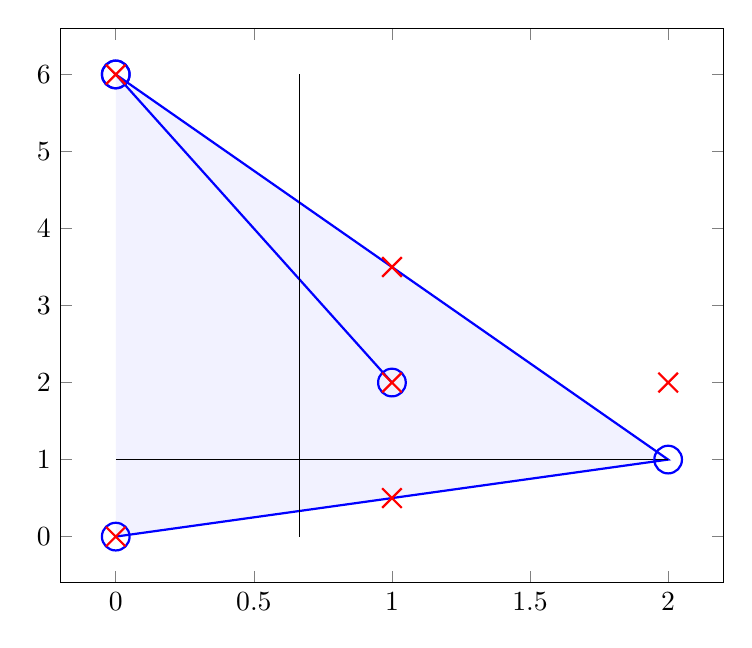
\begin{tikzpicture} 
    \begin{axis}[enlargelimits=0.1]
        \addplot [thick,color=blue,mark=o,fill=blue, 
                    fill opacity=0.05,mark size=5pt]coordinates {
            (0, 0) 
            (2, 1)
            (0, 6)
            (1, 2)
            (0,6)};
        \addplot [only marks,thick,color=red,mark=x,mark size=5pt]coordinates {
            (0, 0) 
            (0, 6)
            (1, 2)
            (1, 3.5)
            (1, 0.5)
            (2, 2)};
            \addplot [
    domain=0:2, 
    samples=100, 
    color=black,
    ]
    {1};
    \addplot +[mark=none, black] coordinates {(2/3, 0) (2/3, 6)};
    \end{axis}
\end{tikzpicture}  
\end{center}
(1, 2) and (1, 3.5) are both Achievable and Enforceable.

\subexercise Find Nash for Payoff of (1,3)
\\\\
\begin{equation} \label{eq1}
\begin{split}
(1,3) & \Rightarrow \begin{cases}
       P + 2Q - 3PQ = 1\\
       2P + Q + 3PQ = 3\\
     \end{cases} \Rightarrow 3P + 3Q = 4 \Rightarrow P = \frac{4}{3} - Q \\
& \Rightarrow \frac{4}{3} - Q + 2Q - 3(\frac{4}{3} - Q)Q = 1 \\
& \Rightarrow \frac{1}{3} + 1Q - 4Q + 3Q^2 = 0 \\
\end{split}
\end{equation}
\begin{equation} \label{eq1}
\begin{split}
& \Rightarrow Q^2 - Q + \frac{1}{9} = 0 \Rightarrow \begin{cases}
       Q = 0.87, P = \frac{4}{3} - 0.87 = 0.46 \textbf{ True Answers}\\
       Q = 0.13, P = \frac{4}{3} - 0.13 = 1.20 \textbf{ Out of Bounds}\\
     \end{cases}\\
& \Rightarrow \begin{cases}
       Q = 0.87\\
       P = 0.46\\
     \end{cases}\\
\end{split}
\end{equation}\\
If anyone derivate from this Nash, other player enforce the minimum payoff for that player as punishment.

\exercise
\subexercise Pure Nash and Payoffs
\\
\begin{equation} \label{eq1}
\begin{split}
(B, L) & \rightarrow (8, 2)\\
(T, R) & \rightarrow (2, 8)
\end{split}
\end{equation}

\subexercise Mixed Nash and Payoffs
\begin{equation} \label{eq1}
\begin{split}
({2 \over 3}B + {1 \over 3} T, {2 \over 3}R + {1 \over 3}L)
\end{split}
\end{equation}
\begin{equation} \label{eq1}
\begin{split}
{4 \over 9}(B,R) + {2 \over 9}(B, L) + {2 \over 9}(T, R) + {1 \over 9}(T, L) = ({44 \over 9}, {44 \over 9})
\end{split}
\end{equation}

\subexercise Correlated Equilibrium and Inequalities
\\\\
General Inequalities:\\ 
\begin{equation} \label{eq1}
\begin{split}
\sum{P(R = a | R_i  = a_i) u_i(a_i, a_{-i}}) \ge \sum{P(R = a | R_i  \neq a_i) u_i({a^\prime}_i, a_{-i}})
\end{split}
\end{equation}
\\
Correlated answer set are below:\\ 
\begin{equation}
    \begin{split}
    C \Rightarrow \begin{cases}
    P_1 \Rightarrow 
     \begin{cases}
            T: P(R = L | R_1  = T) u_1(L, T) + P(R = R | R_1  = T) u_1(R, T) \ge\\
            P(R = L | R_1 = B) u_1(L, B) + P(R = R | R_1  = B) u_1(R, B)\\
            B: P(R = L | R_1  = B) u_1(L, B) + P(R = R | R_1  = B) u_1(R, B) \ge\\
            P(R = L | R_1 = T) u_1(L, T) + P(R = R | R_1  = T) u_1(R, T)\\
     \end{cases}\\
    P_2 \Rightarrow 
     \begin{cases}
            L: P(R = T | R_2  = L) u_2(T, L) + P(R = L | R_1  = B) u_2(L, B) \ge\\
            P(R = R | R_2 = T) u_2(R, T) + P(R = R | R_2  = B) u_2(R, B)\\
            R: P(R = T | R_2  = R) u_2(T, R) + P(R = R | R_1  = B) u_2(R, B) \ge\\
            P(R = L | R_2 = T) u_2(L, T) + P(R = L | R_2  = B) u_2(L, B)\\
     \end{cases}\\
    \end{cases}
    \end{split}
\end{equation}

\begin{equation}
    \begin{split}
    P_{LT}u_1(LT) + P_{RT}u_1(RT) & \ge P_{LB}u_1(LB) + P_{RB}u_1(RB) \\
    P_{LB}u_1(LB) + P_{RB}u_1(RB) & \ge P_{LT}u_1(LT) + P_{RT}u_1(RT) \\
    P_{TL}u_2(LT) + P_{BL}u_2(BL) & \ge P_{TR}u_2(TR) + P_{BR}u_2(BR) \\
    P_{TR}u_2(TR) + P_{BR}u_2(BR) & \ge P_{TL}u_2(LT) + P_{BL}u_2(BL)
    \end{split}
\end{equation}

\begin{equation}
    \begin{split}
    P_{LT}6 + P_{RT}2 & \ge P_{LB}8 + P_{RB}0 \\
    P_{LB}8 + P_{RB}0 & \ge P_{LT}6 + P_{RT}2\\
    P_{TL}6 + P_{BL}2 & \ge P_{TR}8 + P_{BR}0 \\
    P_{TR}8 + P_{BR}0 & \ge P_{TL}6 + P_{BL}2
    \end{split}
\end{equation}

\begin{equation}
    \begin{split}
    6P_{LT} + 2P_{RT} & = 8P_{LB} \\
    6P_{TL} + 2P_{BL} & = 8P_{TR} \\
    P_{TR} + P_{BR} + P_{TL} + P_{BL} & = 1
    \end{split}
\end{equation}
\\
After solving equations
\\
\begin{equation}
    \begin{split}
    P_{LT} = P_{RT} = P_{LB} &= P_c\\
    3P_c + P_{BR}& = 1 \Rightarrow P_{BR} = 1 - 3P_c\\
    u_2(P_c) = u_1(P_c) &= P_c(2 + 8 + 6) = 16P_c, P_c \in [0, 1/3]
    \end{split}
\end{equation}
All values that satisfies above equations is a correlated equilibrium.

\subexercise Correlated Equilibrium with Maximum sum of payoffs
\\
\\
Obviously the maximum sum of payoff happen when $P_c$ equals to ${1 \over 3}$ , which means all $P_{LT} = P_{RT} = P_{LB} = {1 \over 3}$ and  $P_{BR} = 0$

\newpage
\exercise
\subexercise Proof
\\
First we direct proof $\overline{V}(A) = \underline{V}(A)\text{ and  } a_{i^\prime j^\prime }\text{ is Nash }\Rightarrow i^\prime \in i_{sec}\text{, } j^\prime \in j_{sec}$ and then use indirect proof for $\overline{V}(A) = \underline{V}(A)\text{ and  } i^* \in i_{sec}\text{, } j^* \in j_{sec}\Rightarrow a_{i^* j^* }\text{ is Nash}$.
\\
\\
Assume $i^* \in i_{sec}$ and $j^* \in j_{sec}$
\begin{equation}
    \begin{split}
    a_{i^\prime j^\prime} \text{is Nash} & \Rightarrow \begin{cases}
        a_{i^\prime j^\prime} = \min_i{a_{j^\prime}} \Rightarrow a_{i^\prime j^\prime} = a_{i^* j^\prime}\\
        a_{i^\prime j^\prime} = \max_j{a_{i^\prime}} \Rightarrow a_{i^\prime j^\prime} = a_{i^\prime j^*}
    \end{cases}\\
    \overline{V}(A) = \underline{V}(A) & \Rightarrow \max_j{a_{i^* j}} = \min_i{a_{i j^*}} = a_{i^* j^*}\\
    \begin{cases}
        a_{i^* j^*} \ge a_{i^* j^\prime}\\
        a_{i^* j^*} \le a_{i^\prime j^*}
    \end{cases} & \Rightarrow \begin{cases}
        a_{i^* j^*} \ge a_{i^\prime j^\prime}\\
        a_{i^* j^*} \le a_{i^\prime j^\prime}
    \end{cases} \Rightarrow a_{i^*, j^*} =  a_{i^\prime j^\prime}
    \end{split}
\end{equation}

\begin{equation}
    \begin{split}
        a_{i^\prime j^\prime} & = a_{i^*, j^*} \\
        \min_i{a_{i j^\prime}} & = min_i{a_{i j^*}}\\
        \Rightarrow \min_i{a_{i j^\prime}} & \ge \min_i{a_{ij}}\\
        \Rightarrow j\prime & \in j_{sec}
    \end{split}
\end{equation}

\begin{equation}
    \begin{split}
        a_{i^\prime j^\prime} & = a_{i^*, j^*} \\
        \max_j{a_{i\prime i}} & = max_j{a_{i^* j}}\\
        \Rightarrow \max_j{a_{i^\prime j}} & \le \max_j{a_{ij}}\\
        \Rightarrow i\prime & \in i_{sec}
    \end{split}
\end{equation}
\\
\\
For Proving $[\overline{V}(A) = \underline{V}(A)\text{ and  } i^* \in i_{sec}\text{, } j^* \in j_{sec} \Rightarrow a_{i^* j^* }\text{ is Nash}]$, let's assume that there are such $i^*$ and $j^*$ which satisfies player security strategy but are not Nash equilibrium. In this case if a Nash equilibrium exists, we assume in $(i^\prime, j^\prime)$ then $a_{i^\prime j^\prime}$ should be less than $a_{i^*, j^\prime}$ and more than $a_{i^\prime j^*}$, Which leads to $i^*$ and $j^*$ are no longer a security strategies and it contrast with our primary assumptions, so $(i^*, j^*)$ should be a Nash equilibrium.

\subexercise Proof

\begin{equation}
    \begin{split}
        a_{i_1j_1} & \Rightarrow \begin{cases}
        a_{i_1j_1} \le min_i{a_{ij_1}} \Rightarrow a_{i_1j_1} \le a_{i_2j_1}\\
        a_{i_1j_1} \ge max_j{a_{i_1j}} \Rightarrow a_{i_1j_1} \ge a_{i_1j_2}
        \end{cases}\\
        a_{i_2j_2} & \Rightarrow \begin{cases}
        a_{i_2j_2} \le min_i{a_{ij_2}} \Rightarrow a_{i_2j_2} \le a_{i_1j_2}\\
        a_{i_2j_2} \ge max_j{a_{i_2j}} \Rightarrow a_{i_2j_2} \ge a_{i_2j_1}
        \end{cases}
    \end{split}
\end{equation}

\begin{equation}
    \begin{split}
         & a_{i_1j_1} \le  a_{i_2j_1} \le  a_{i_2j_2} \le  a_{i_1j_2} \le  a_{i_1j_1}\\
         \Rightarrow & a_{i_1j_1} =  a_{i_2j_1} =  a_{i_2j_2} =  a_{i_1j_2}\\
         \Rightarrow & \text{Therefore, all four points are Nash equilibrium}
    \end{split}
\end{equation}

\newpage
\exercise

\subexercise Disproof.
It might fall into a loop depending of initial actions and size of the game. (For 2 by 2 it works fine)\\
Example is below table when non of start actions are 1.\\
\begin{center}
\begin{tabular}{ |c|c|c|c| } 
\hline 
 & 0 & 1 & 2 \\
\hline
\multirow 0 & 2 , 0 & 1 , 1 & 0 , 2 \\ 
\hline
1 & 1 , 1 & 3 , 3 & 1 , 1 \\ 
\hline
2 & 0 , 2 & 1 , 1 & 2 , 0 \\ 
\hline
\end{tabular}    
\end{center}

\subexercise New Algorithm.\\\\

Assume we have a two-player normal form game in which players has $n_i$ actions.
We can use dynamic programming approach and split the game of $n_1 * n_2$ to a 4 sub-game of $\lceil {n_1 \over 2} \rceil * \lceil {n_2 \over 2} \rceil$ and after solving each sub-game we might reach a Nash for each of them with two corresponding actions, then we reduce our four answers to a new $2 * 2$ game and find the Nash for $2*2$ with BestResponce-Algorithm which shown in last part.

\begin{minted}{python}
def find_nash_final(G):
    actions = []  # Two corresponding action which leads to Nash
    value = 0.0  # value of the Nash
    # Find Nash by given algorithm using BestResponse
    return actions, value
def find_nash(G):
    n1 = len(G); n2 = len(G[0])
    if n1 < 3 or n2 < 3:
        return find_nash_final(G)
    else:
        half_n1 = floor(n1 / 2); half_n2 = floor(n2 / 2)
        # Create four sub-game
        sub_game = [
            G[:half_n1, :half_n2],
            G[:half_n1, half_n2:],
            G[half_n1:, :half_n2],
            G[half_n1:, half_n2:]
        ]
        # Find Nash of each sub-game
        actions = []; values = []
        for game in sub_game:
            act, val = find_nash(game)
            actions.append(act)
            values.append(val)
        # Create the final game with four state
        final_game = [
            [values[1], values[2]],
            [values[3], values[4]]
        ]
        # Solve the final game and return Nash Equilibrium actions and
        act, val = find_nash_final(final_game)
        return actions[act[0] * 2 + act[1]], val
\end{minted}{python}

\proof Assume a pure Nash Equilibrium exists for this game, so it will remains a Nash in any sub-game of this game which contain that state. This algorithm have two phase of divide and merge, which will be discussed in below.\\\\
(1) In divide phase, after we recursively divide the game to sub-games with size less than 3, we have the opportunity to solve them. In this phase the general pure Nash will surely be selected as Nash of its own sub-game and send to next level. (Definition of pure Nash)
\\\\
(2) In merge phase, we create a new sub-game of with four winner state of child sub-games and the general Nash from previous step will be shown in a new sub-game and continue to winning till reach the final game.
\\\\
Therefore, at the end the general pure Nash will not get lost, and we find it's values and corresponding actions.
\\\\
\textbf{Calculation Time-Complexity}\\
Assume player 1 has $N$ and player 2 has $M$ actions and $N \ge M$.\\\\
Sub Game(Case 1): $T_{nash}(0*0) = 0, T_{nash}(1*1) = 0, T_{nash}(2*2) = 4$\\
Sub Game(Case 2): $T_{nash}(0*N) = 0, T_{nash}(1*N) = N, T_{nash}(2*N) = 2*N$\\
\\
Sub Game Order Worst: $O(SubGame) = O(N)$\\
Sub Game Order Best: $O(SubGame) = constant $\\\\
Divide: $T_{divide}(MN) = 4T_{divede}(MN/4) = 4^{\log_4{MN}}*T_{subgame} = MN*T_{subgame}$\\\\
Total Order Worst: $O(Game) =  O(MN) * O(N) = O(MN^2)$\\
Total Order Best: $O(Game) = O(MN) * constant = O(MN)$\\\\
Total Order $M = N$: $O(Game) = O(N^2) * constant = O(N^2)$\\\\

\end{document}
